\section{Alfadian Owen}



 
 
\subsection{Sejarah python}


\qquad Bahasa pemrograman Python adalah bahasa yang dibuat oleh seorang keturunan Belanda yaitu Guido van Rossum. Awalnya, pembuatan bahasa pemrograman ini adalah untuk membuat skrip bahasa tingkat tinggi pada sebuah sistem operasi yang terdistribusi Amoeba. Python telah digunakan oleh beberapa pengembang dan bahkan digunakan oleh beberapa perusahaan untuk pembuatan perangkat lunak komersial.


\subsection{Instalasi Anaconda}
\begin{enumerate}
\item Download Terlebih dahulu aplikasi anaconda yang ada di https://www.anaconda.com/distribution/ 
\item Setelah download anda selesai, buka file yang anda download tadi
\item Klik next
\begin{figure}[H]
\centering
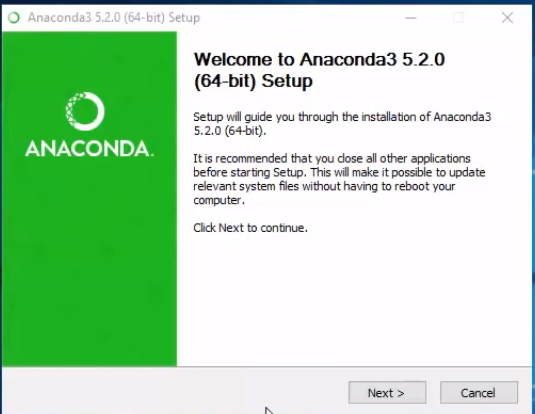
\includegraphics[width=6cm,height=6cm]{figures/gambar1.png}
\caption{Klik Next}
\label{akhir}
\end{figure}
\item Klik I Agree
\begin{figure}[H]
\centering
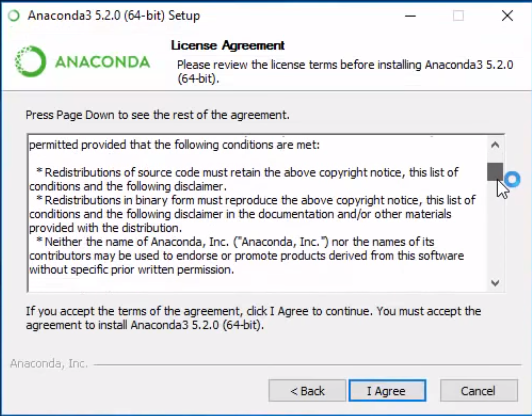
\includegraphics[width=6cm,height=6cm]{figures/gambar2.png}
\caption{Klik I Agree}
\label{akhir}
\end{figure}
\item Pilih sesuai yang anda inginkan tetapi saya merekomendasikan all user agar dapat dipakai oleh semua user
\begin{figure}[H]
\centering
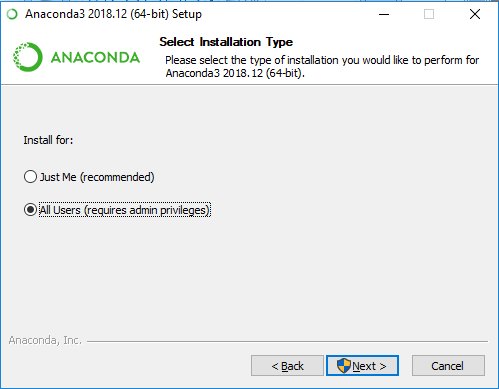
\includegraphics[width=6cm,height=6cm]{figures/gambar3.png}
\caption{Pilih sesuai yang anda inginkan}
\label{akhir}
\end{figure}
\item Pilih directory tempat anaconda akan diinstall lalu next
\begin{figure}[H]
\centering
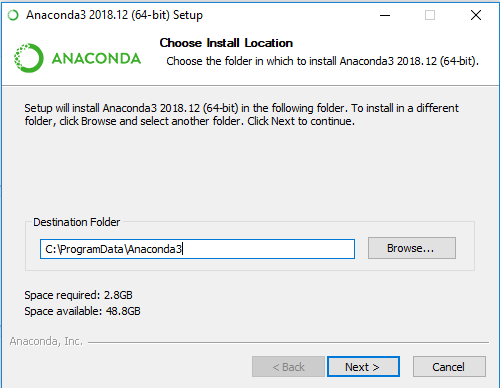
\includegraphics[width=6cm,height=6cm]{figures/gambar4.png}
\caption{Directory tempat anaconda akan diinstall}
\label{akhir}
\end{figure}
\item jika anda belum pernah menginstall python maka checklist keduanya dan jika anda sudah menginstall python maka checklist yang paling bawah saja
\begin{figure}[!htbp]
\centering
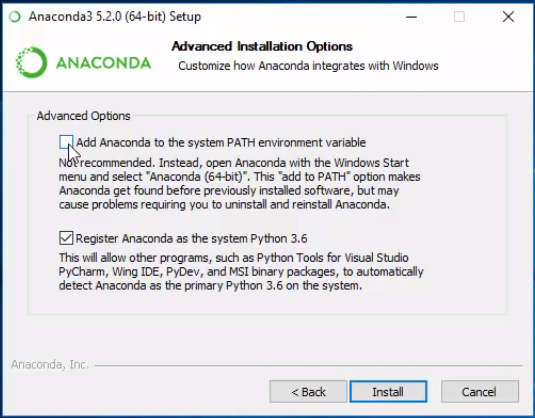
\includegraphics[width=6cm,height=6cm]{figures/gambar5.png}
\caption{Opsi Register}
\label{akhir}
\end{figure}
\item Tunggu hingga proses selesai lalu next
\begin{figure}[H]
\centering
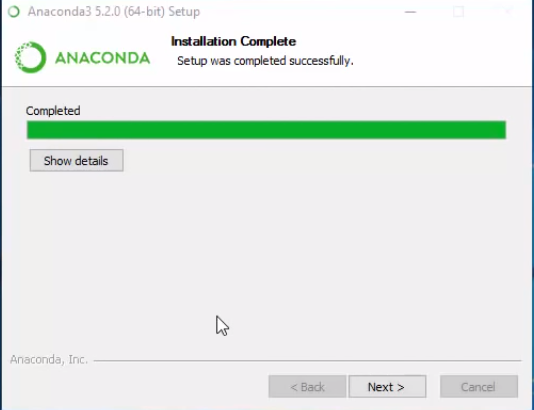
\includegraphics[width=6cm,height=6cm]{figures/gambar6.png}
\caption{Tunggu hingga selesai}
\label{akhir}
\end{figure}
\item Opsi tambahan untuk instal visual studio code, skip saja
\begin{figure}[H]
\centering
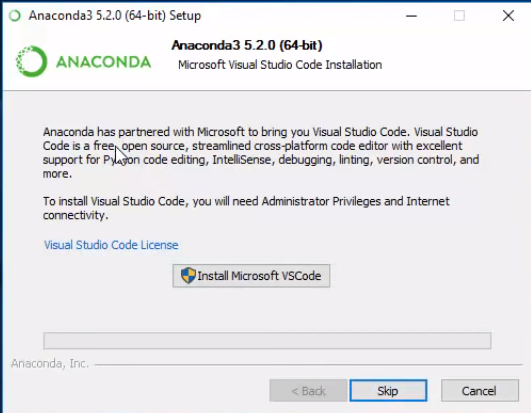
\includegraphics[width=6cm,height=6cm]{figures/gambar7.png}
\caption{Opsi Tambahan}
\label{akhir}
\end{figure}
\item uncheck semua dan click finish
\begin{figure}[H]
\centering
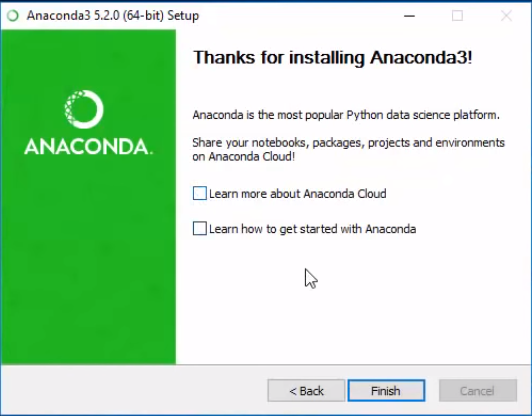
\includegraphics[width=6cm,height=6cm]{figures/gambar8.png}
\caption{Finish}
\label{akhir}
\end{figure}
\end{enumerate}

\subsection{Spyder}
\begin{enumerate}
\item Setelah install anaconda, buka aplikasinya.
\item Biasanya spyder sudah terinstall dengan anaconda, klik launch pada spyder
\begin{figure}[H]
\centering
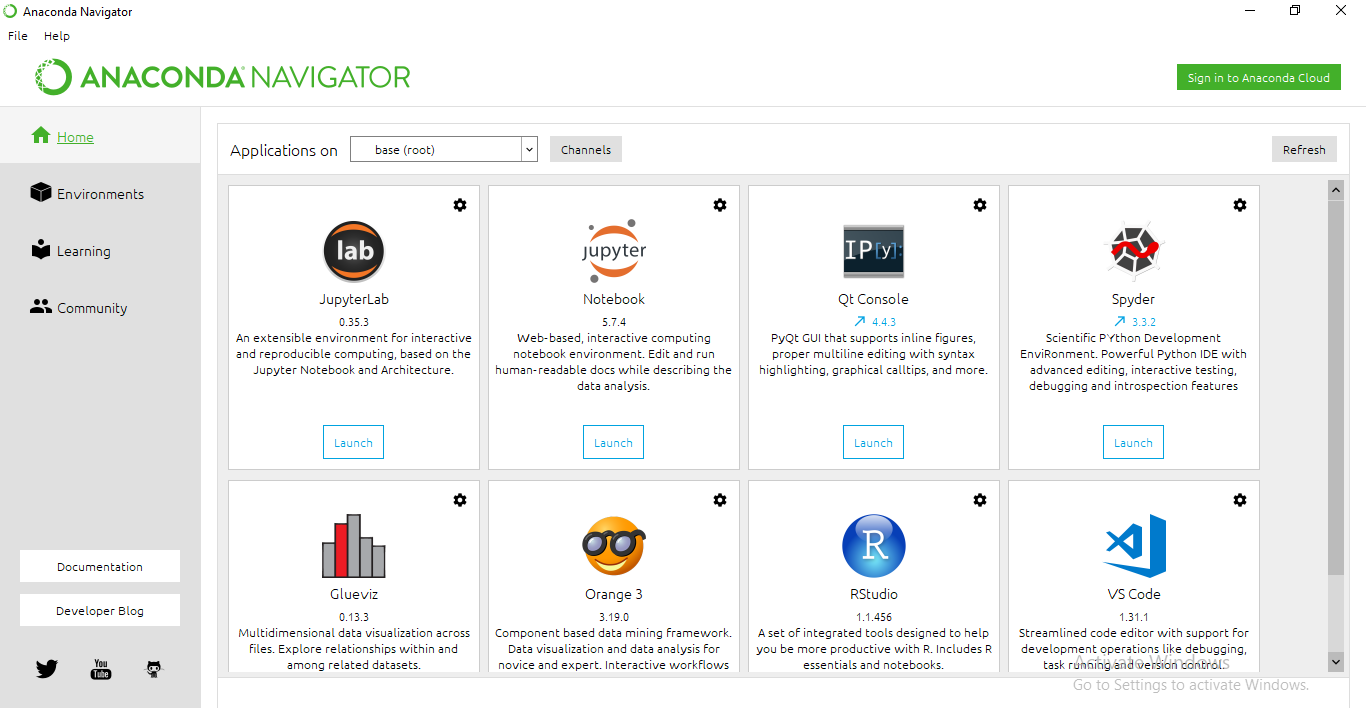
\includegraphics[width=6cm,height=6cm]{figures/gambar9.png}
\caption{Menu Utama Anaconda}
\label{Spyder}
\end{figure}
\item selesai, jika ingin melakukan percobaan maka ketik yang ada di bagian kiri lalu run atau F5
\begin{figure}[H]
\centering
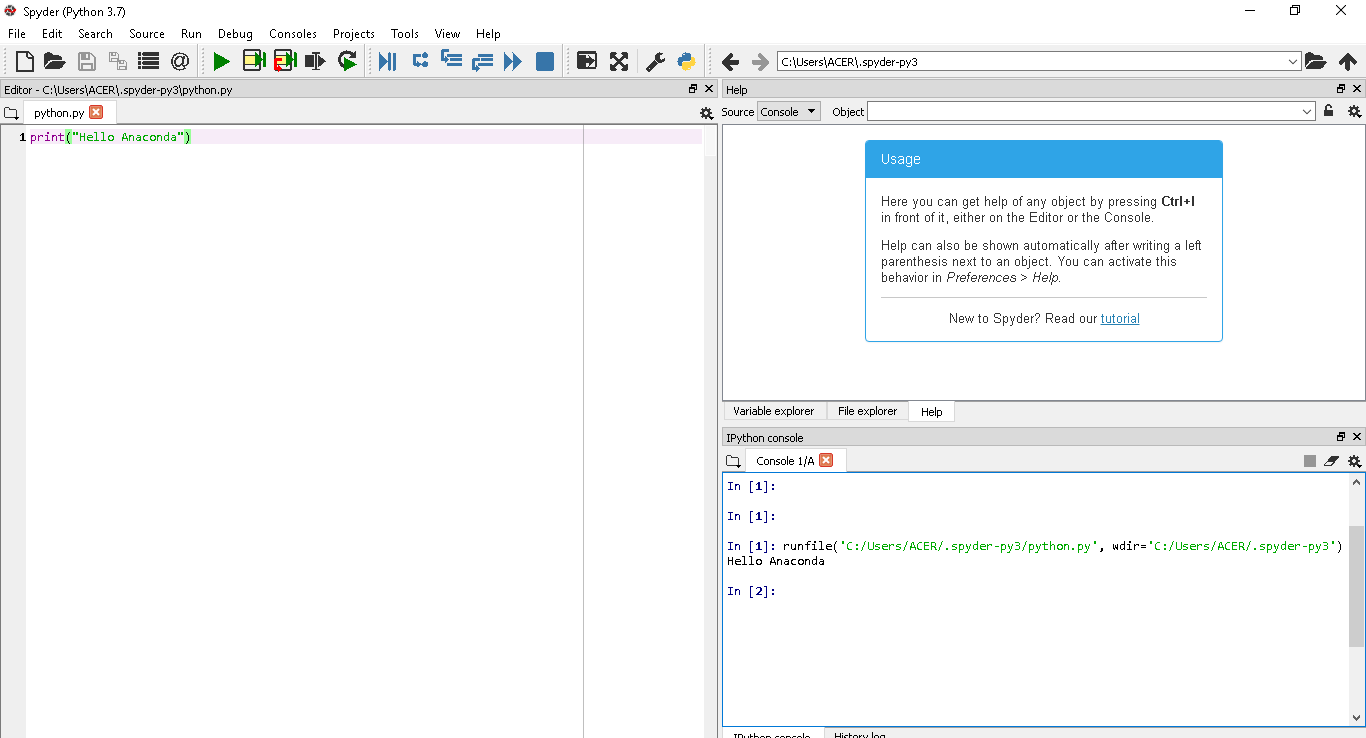
\includegraphics[width=6cm,height=6cm]{figures/10.png}
\caption{Spyder}
\label{akhir}
\end{figure}




\end{enumerate}
